\subsection{Event selection} \label{sec:WBoson_Analysis_Selection}


The signal events, determined by the process \WToMuNu, are characterised by a high-\pt muon and the presence of missing transverse momentum \ptmiss, originated from the undetected neutrino. Events with similar characteristics can be produced by other background processes, such as semi-leptonic decays of hadrons formed within jets or dilepton decays of \Z bosons. This section explain the different selections implemented to suppress the background while keeping the signal.

%%------------------------------------------------------------%%
\subsubsection{\RunpPb global filter} \label{sec:WBoson_Analysis_Selection_EventFilter}

In order to ensure that the samples are not contaminated by events not originating from the inelastic hadronic collisions, a standard \RunpPb Global Event Filter (GEF) is applied. The different selections included in the \RunpPb GEF are described below:

\begin{itemize}
 \item Primary vertex filter: requires the presence of a primary vertex reconstructed from at least two tracks, within a longitudinal (transverse) distance of \SI{25}{\cm} (\SI{2}{\cm}) of the nominal interaction point. This selection reduces the contamination from non-collision backgrounds, such as cosmic-ray muons or accelerator-induced particles.
 \item HF coincidence filter: requires at least one tower on each side of the interaction point in the Hadron-Forward calorimeter, with an energy deposit per tower of at least \SI{3}{\GeV}. This filter rejects events from  electronic noise and beam-beam electromagnetic interactions.
 \item Beam-scraping filter: requires at least 25$\%$ of tracks in the event to be high quality tracks. This requirement is used to further suppress the contribution from beam-related backgrounds, such as beam-gas interactions and beam-halo events.
\end{itemize}

The impact of the GEF was checked both in data and simulation. Only 0.08$\%$ of events in data and 0.06$\%$ of events in the \WToMuNu simulation, passing all analysis selections summarized in \sect{sec:WBoson_Analysis_Selection_WSelection}, were removed by the filter.


%%------------------------------------------------------------%%
\subsubsection{Trigger} \label{sec:WBoson_Analysis_Selection_Trigger}

The events used in this analysis were selected online with the HLT trigger \verb#HLT_PAL3Mu12#. This trigger requires a fully reconstructed L3 muon with $\pt > 12$~\GeVc. The HLT trigger was seeded with the L1 trigger path \verb#L1_SingleMu7#, which pass events with at least one L1 muon with $\pt > 7$~\GeVc. It is to be noted that only muons of \pt greater than 25~\GeVc are considered in the offline analysis, and such trigger is extremely efficient for those.

A reconstructed muon is considered matched to the trigger, if it matches the L3 muon that fired the trigger. The matching criteria between the reconstructed muon and the L3 muon requires:

\begin{equation}
 \Delta{R}\left(\mu_{\text{reco}} , \mu_{\text{HLT}}\right) = \sqrt{\left(\eta^{\mu}_{reco} - \eta^{\mu}_{HLT}\right)^{2} + \left(\phi^{\mu}_{reco} - \phi^{\mu}_{HLT}\right)^{2}} < 0.1
\end{equation}

The $\Delta{R} < 0.1$ matching criteria is a standard threshold commonly used in CMS analyses employing L3 muon triggers~\cite{MuonReco}. It has been selected taking into account the $\eta$ and $\phi$ resolutions of muon tracks reconstructed with the HLT L3 and offline muon algorithms.

%%------------------------------------------------------------%%
\subsubsection{Muon selection} \label{sec:WBoson_Analysis_Selection_MuonIdentification}

Muon candidates are identified using a standard \textit{tight} selection, optimised for muons with high \pt. The tight selection requires muon candidates to be reconstructed globally from hits in the muon stations and the tracker, be identified with the PF algorithm~\cite{PF_Reco} and pass the following criteria:

\begin{itemize}
\item The muon track fit has at least a $\chi^{2}$ per degree of freedom less than ten, ensuring a minimal fit quality.
\item The muon track segments are matched to at least two muon stations, making the selection consistent with the muon trigger logic.
\item The transverse impact parameter (longitudinal distance) of the muon track is consistent with the primary vertex within \SI{2}{\mm} (\SI{5}{\mm}), to reduce the background from cosmic rays and muon decays in flight (e.g. from pion, kaon and heavy-flavour hadron decays). 
\item The muon track has at least one hit in the pixel detector to further suppress muons from decays in flight.
\item The muon track includes hits in at least six inner-tracker layers to guarantee a good \pt measurement.
\end{itemize}

Apart from the \textit{tight} identification criteria, muon candidates are also required to be isolated in order to reduce the proportion of muons coming from jets. Muons are considered isolated if the sum of the \pt of all PF-identified photons, charged hadrons and neutral hadrons, within a cone of $\Delta{R}\left(\mu , \text{PF}\right) < 0.3$, is less than 15$\%$ of the muon \ptMu. The muon isolation variable is thus defined as:

\begin{equation}
 \iso = \left(\sum_{\text{charged hadrons}}^{\Delta{\text{R}}<0.3} \pt + \sum_{\text{neutral hadrons}}^{\Delta{\text{R}}<0.3} \pt + \sum_{\text{photons}}^{\Delta{\text{R}}<0.3} \pt\right)\bigg/\ptMu
 \label{eq:MuonIsolation}
\end{equation}

Finally, muon candidates are required to have $\pt > 25$~\GeVc and be within $|\etaLAB| < 2.4$. If more than one muon is found with $\pt > 25$~\GeVc and passing the identification criteria in a given event, then the corresponding muon with the highest \pt is used. This happens in 3\% of events in data but are later suppressed down to 0.001\% of events with the \DYToMuMu veto described in the next section.


%%------------------------------------------------------------%%
\subsubsection{\DYToMuMu veto} \label{sec:WBoson_Analysis_Selection_DrellYanVeto}

A veto is applied to suppress the contribution from \DYToMuMu background events. This veto consists in removing events that contain at least two opposite-sign muons with $\pt > 15$~\GeVc, each passing the muon identification and isolation criteria.

The probability that \DYToMuMu events survive the veto is checked using simulation. The denominator of the \DYToMuMu veto efficiency is filled with muons passing the signal selection criteria summarised in the next section, while the numerator is filled with the same muons as long as the event passes the \DYToMuMu veto. The simulated survival probability is shown in \fig{fig:DrellYanVetoZEfficiency2D}. As can be observed, most of the \DYToMuMu events that survive the veto mainly contributes in the forward pseudorapidity region, where one of the muons from the \DY-boson decay escapes the detector.

\begin{figure}[htb]
 \centering
 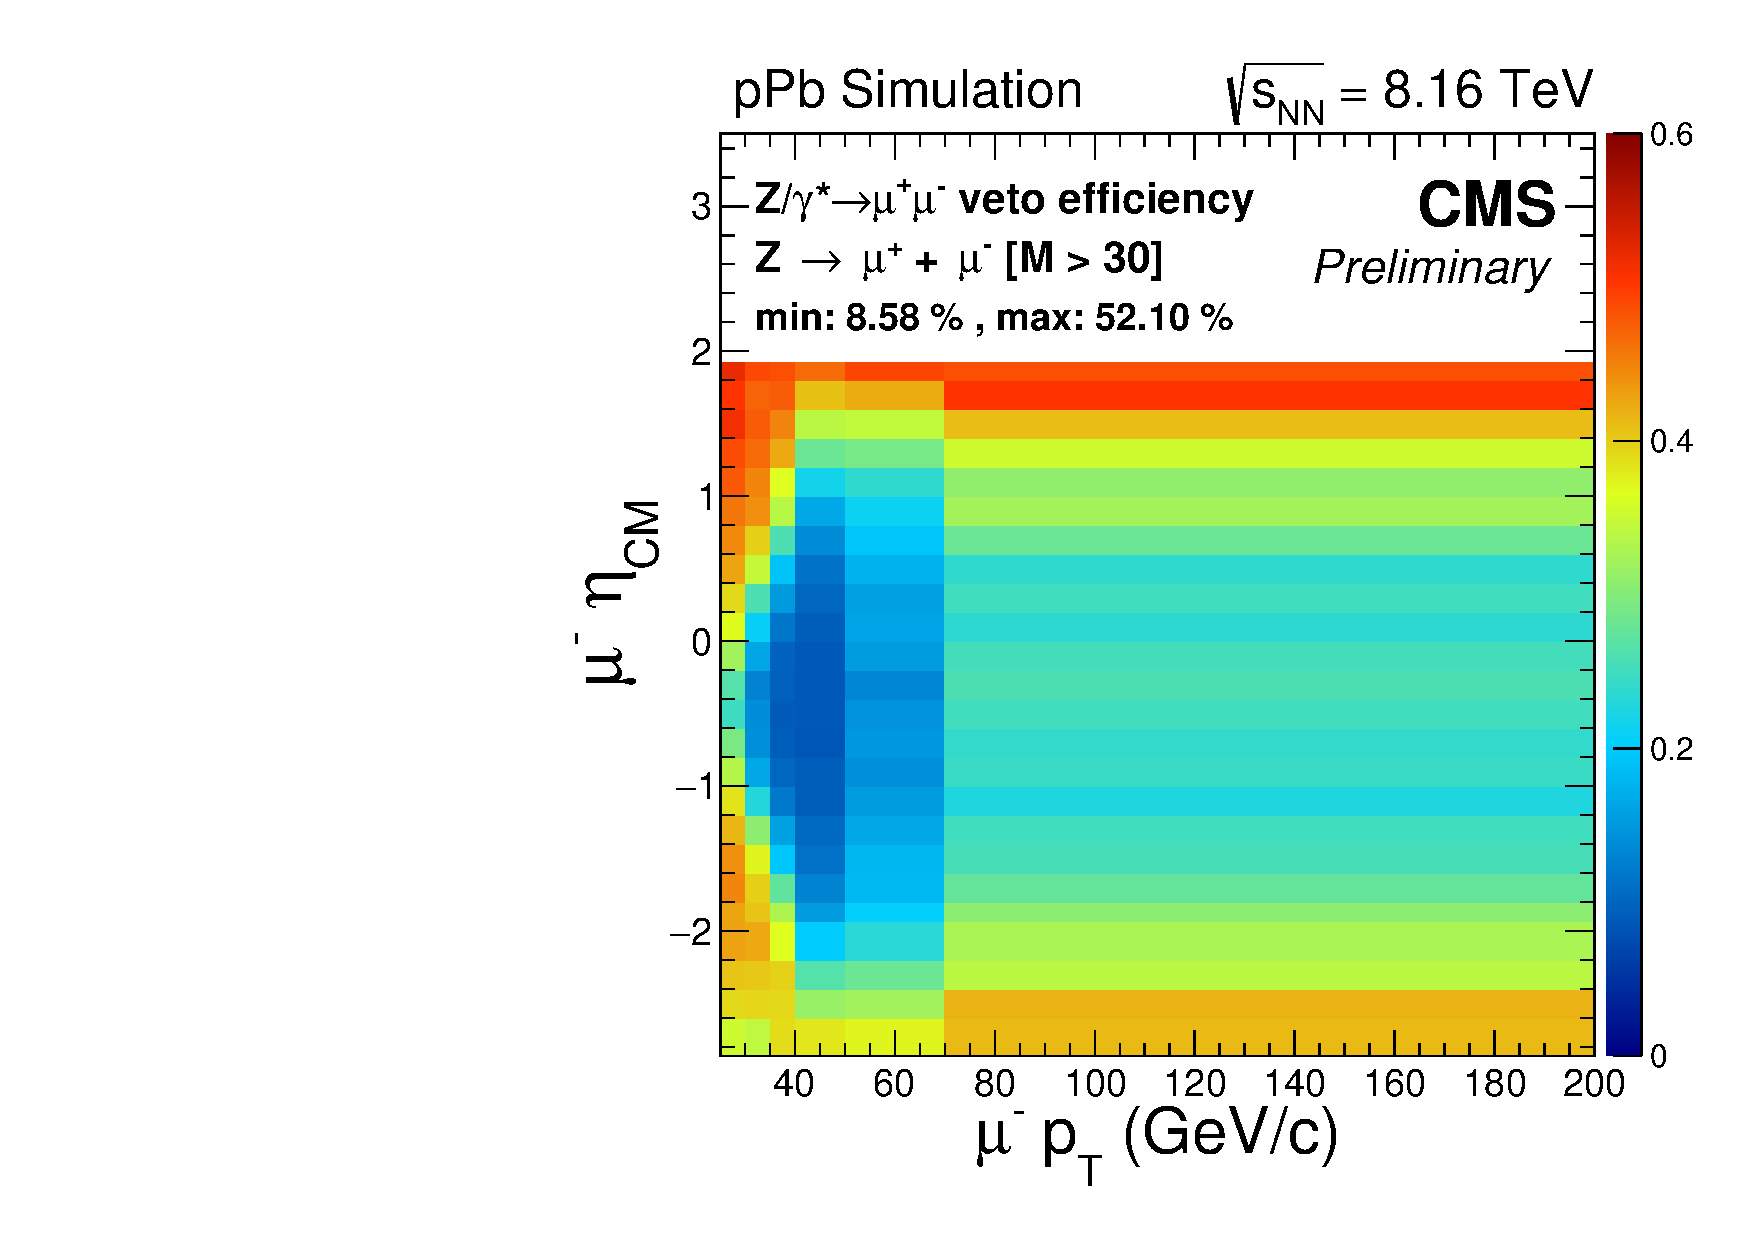
\includegraphics[width=0.45\textwidth]{Figures/WBoson/Analysis/Efficiency/eff2D_Pt_EtaCM_MC_ZToMuMu_M_30_Inf_PA_Minus_DrellYanVeto}
 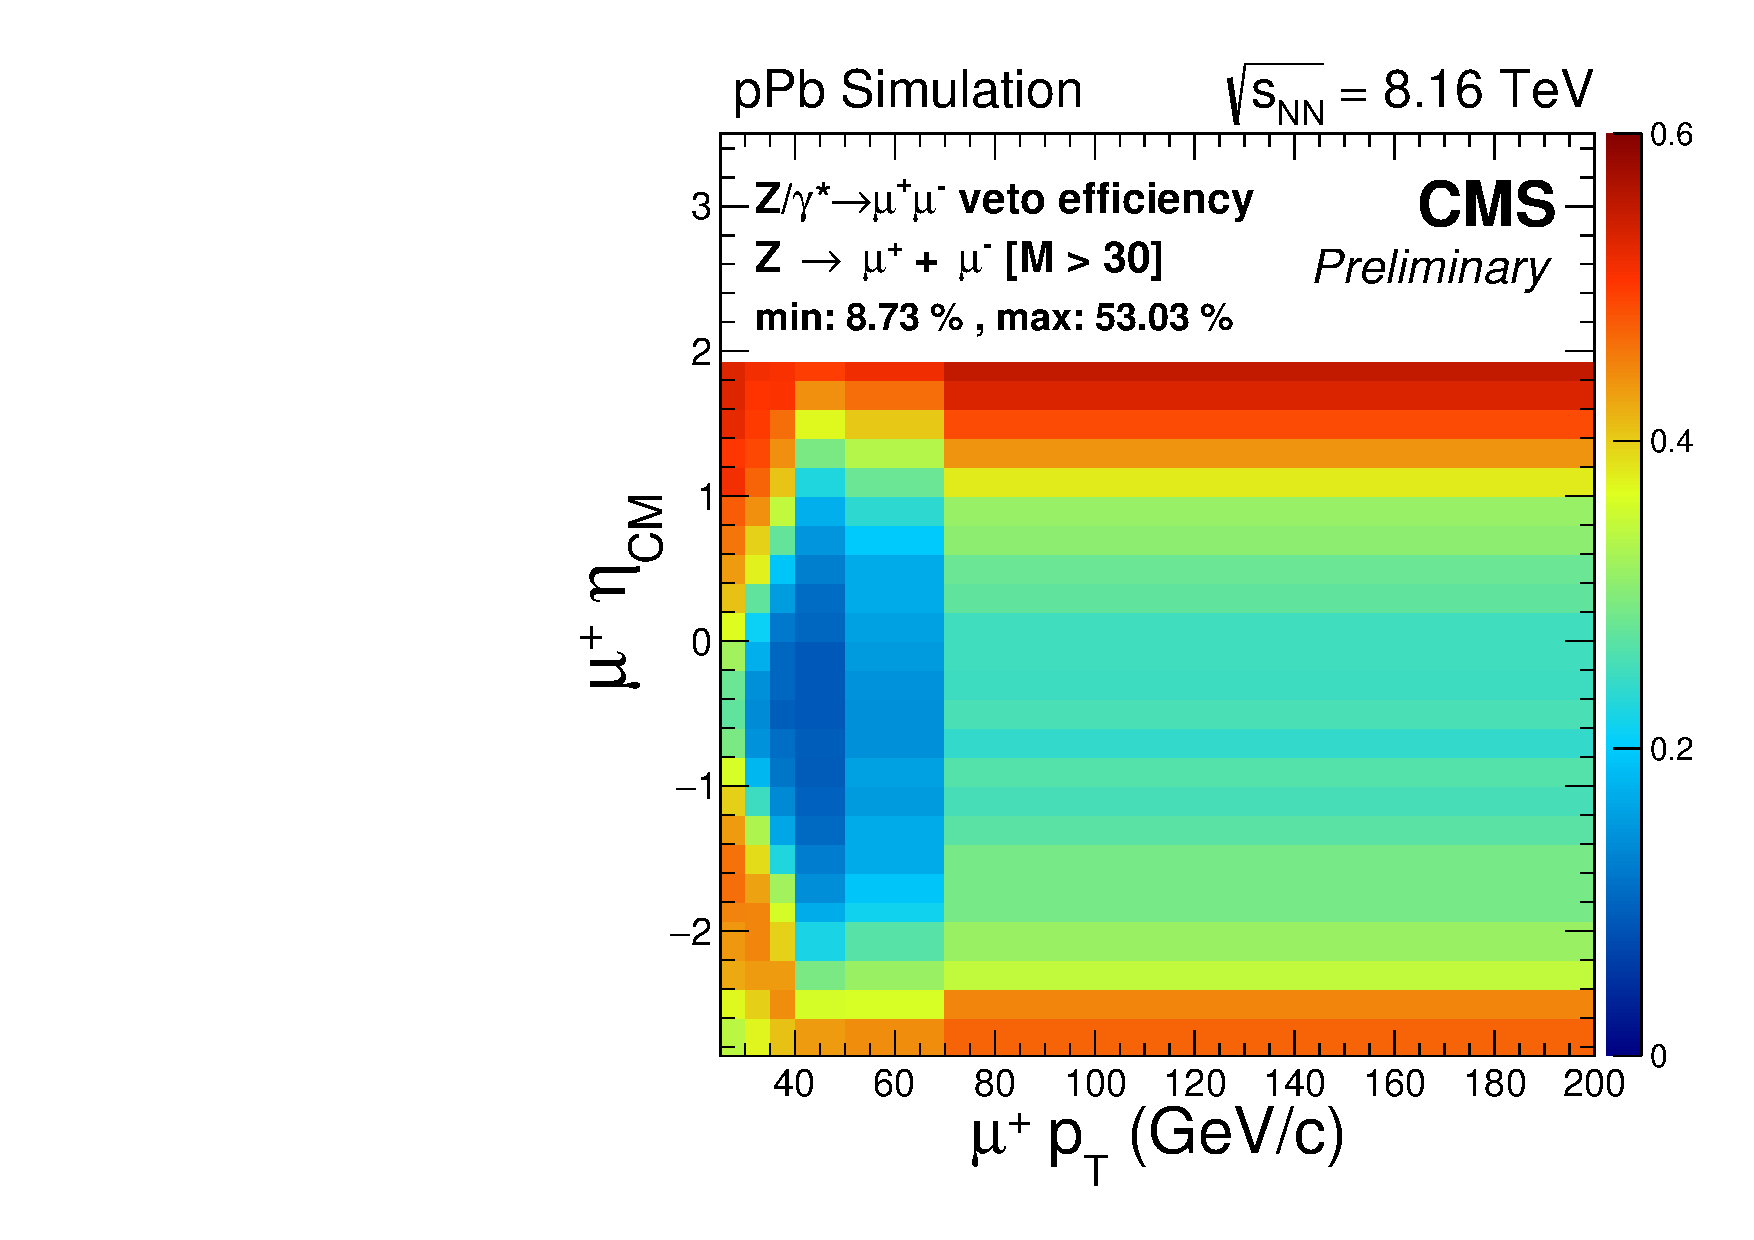
\includegraphics[width=0.45	\textwidth]{Figures/WBoson/Analysis/Efficiency/eff2D_Pt_EtaCM_MC_ZToMuMu_M_30_Inf_PA_Plus_DrellYanVeto}
 \caption{Survival probability of single muons from a \DYToMuMu (M$ > 30$~\GeVcc) simulation, as a function of the muon \etaMuCM and \ptMu, separated in negative (left) and positive (right) charged muons. Muons are required to have $\pt > 25$~\GeVc and $|\eta| < 2.4$, match the trigger and pass the isolation and identification criteria.}
 \label{fig:DrellYanVetoZEfficiency2D}
\end{figure}


%%------------------------------------------------------------%%
\subsubsection{Event selection summary} \label{sec:WBoson_Analysis_Selection_WSelection}

In summary, the signal selection consists of the detection of a high-\pt muon, passing the identification criteria detailed in \sect{sec:WBoson_Analysis_Selection_MuonIdentification}. The muon candidate is required to have $\pt > 25$~\GeVc, be isolated and match the trigger (see \sect{sec:WBoson_Analysis_Selection_Trigger}). The events entering the signal region are also required to satisfy the \RunpPb global event filter (\sect{sec:WBoson_Analysis_Selection_EventFilter}) and the \DYToMuMu veto (\sect{sec:WBoson_Analysis_Selection_DrellYanVeto}).

The other signature of a \WToMuNu event is a high-\pt neutrino, estimated through the \ptmiss. No explicit selection is applied on the missing transverse momentum. The \ptmiss is directly used to extract the event yields by fitting the signal and background components. Apart from the main signal sample, two more samples are used:
\begin{itemize}
 \item \ZToMuMu control sample: selects \ZToMuMu events by reverting the \DYToMuMu veto and selecting \mumu pairs with invariant mass within the \Z-boson mass window. Used to derive corrections for the weak boson \pt (\sect{sec:WBoson_Analysis_Corrections_WeakBosonPTReweighing}) and the \ptmiss (\sect{sec:WBoson_Analysis_Corrections_MET}).
 \item \QCD jet control sample: selects non-isolated muon events by reverting the muon isolation cut. Used to determine the shape of the QCD jet background from data.
\end{itemize}

The conditions used to define the signal and control regions of interest are illustrated in \fig{fig:EventSelectionDiagram}.

\begin{figure}[htb]
 \centering
 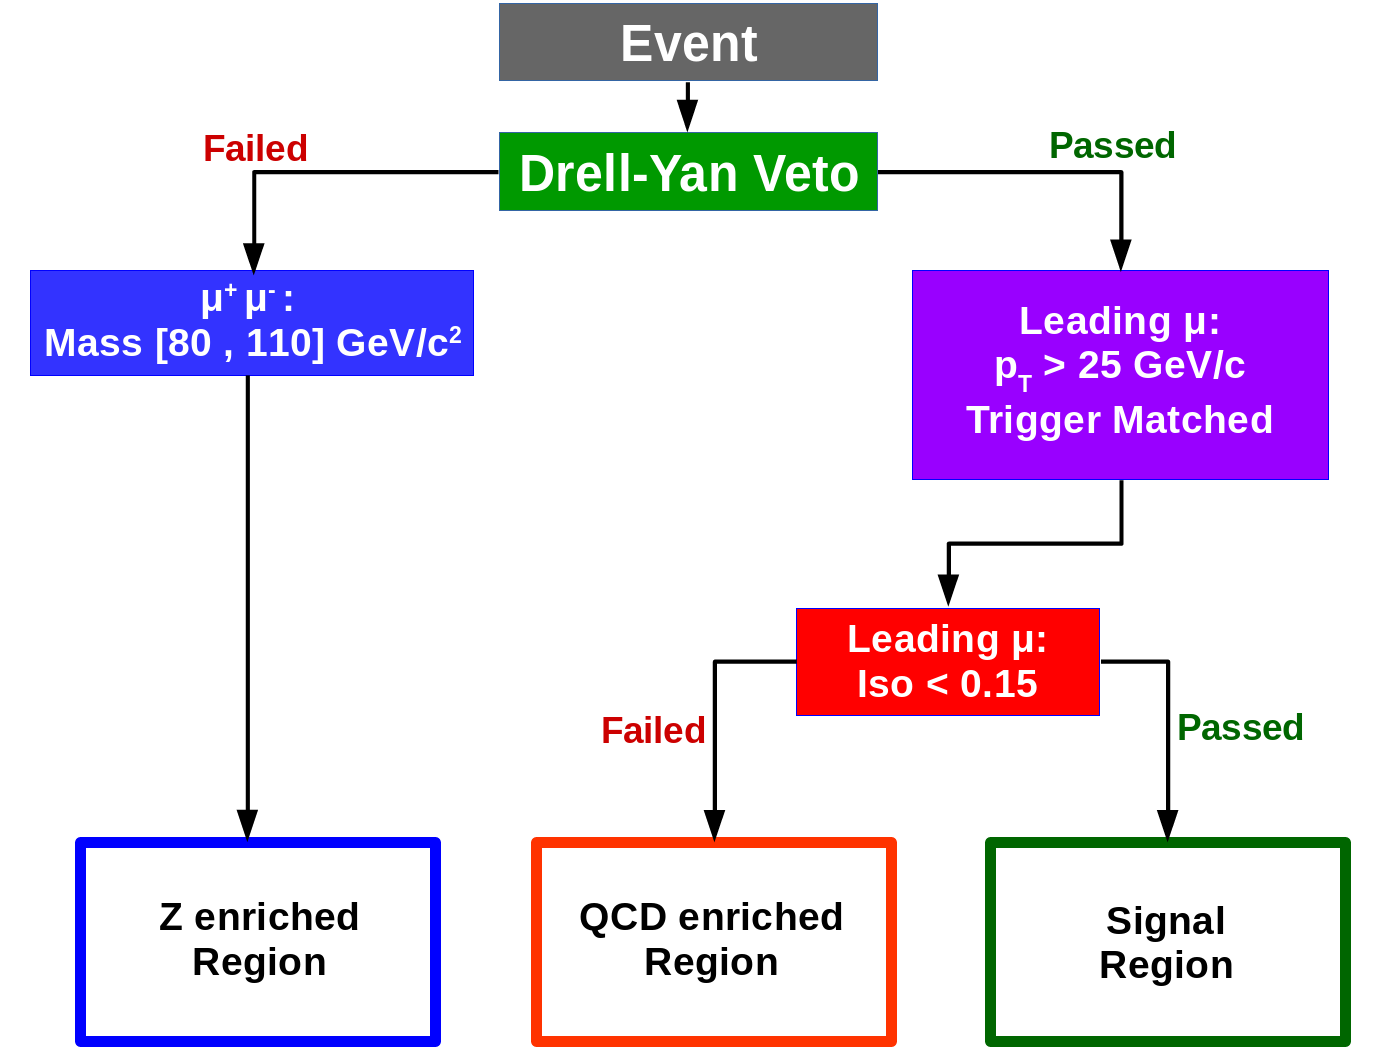
\includegraphics[width=0.8\textwidth]{Figures/WBoson/Analysis/EventSelection/FlowChar.png}
 \caption{Flowchart illustrating the way the events are classified.}
 \label{fig:EventSelectionDiagram}
\end{figure}

% END OF SUBSECTION
